%!TEX root = ../docu.tex
\section{Entwicklung}
\subsection{Benutzeroberfläsche}
\subsection{Einstellungen}
Das einstellungsmenü soll in jedem zustand der application ereichbar sein. der einzige ort an dem dies möglich sit ist das menü. hier ist nciht von einem implementierten menü die reden. dieses menü ist in jeder applikation erreichbar und wird durch das betriebssystem bereitgestellt.

druck ein benutzer die menü taste welche sich an jedem gerät befindet welches android als betriebssystem verwendet so öffnet sich ein eine menü schnittstelle welche durhc den entwickler miteinträgen befüllt werden kann um bestimmte funktionen bereitzustellen. eine typishce funktion ist die bereitstelleung der einstellungsseite.

die konfiguration für die naziege welche einstellungsmöglichkeitem dem nutzer zur verfügung gestellt wird erfolgt über eine XML datei. in älteren API versionen wurde dies noch durch klassen realisiert.diese klassen und emhtoden sind in den version ab android version 4 veraltet und sollten nciht mehr verwendet werden.

die erwähnte XMl datei wird nun durhc bestimmte regler und kontrollstrukturen bestückt. diese strukturen werden durch ids validiert. ihre werte können durhc eine abfrage aus der anwendung herraus ausgelesen werden.

sollten keine geeigneten vorgefertigte kontrollstrukturen wie zum beispiel radiu button und checkboxen vorhanden sein so können eigene strukturen eingebettet werden.

im kontrten beispiel existiert keine struktur für das speicher und durchsuchen  eines ordnerpfades. dieser \textit{FilePicker} wurde daher eigens implementiert und kann aus dem einstellungsmenü aufgerufen werden.

\begin{center}
\begin{figure}
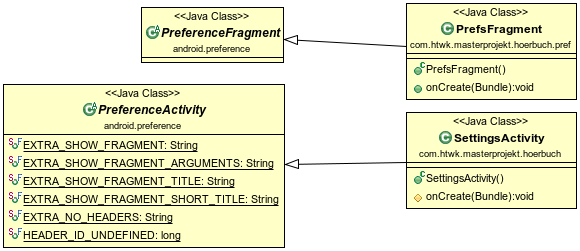
\includegraphics[scale=0.7]{images/settings}
\caption{Klassen für die Implementierung der Einstellungen}
\label{settings}
\end{figure}
\end{center}

wurde der gewünschte ordner gefunden kann dieser in in den einstlelungen gespeichert werden. alle anderen komponenten der anwendung können nun auf diese einstellungen zugreifen.

dies wird über den \textit{PreferenceManager} realisiert. er benötigt für die abfrage des wertes jediglicht die id der einstellung, welche abgefragt werden soll. zu sicherheit wird bei der abfrage ein standrat wert angebgeben im falle das die eisntellung nciht geufndne oder ausgelesen werden konnte. die einmal eingetragen einstellungen sind jederzeit abrufbar und auch nach beenden der applikation imemrnoch vorhanden.

Die Abbildung \ref{settings} zeigt die benötigeten Klassen für die Implementierung der funktionalität der einstellungen.

\subsection{Datenbank}
\subsubsection{Grundlagen}
Dass Android eine schnittstelle für SQlite dantenbanken anbietet wurde schön in einem vorrausgestellten Kpitel behandelt \ref{Datenbankstrukturen}. Anshcließend soll erläutert werden wie man diese anbiendung benutzt und wie daten gespeichert und abgefragt werden können.

Zunächst benötigen wir eine Klasse welche die API klasse \textit{SQLiteOpenHelper} erweitert. Die entstehende klasse bildet nun die schnittstelle unser applikation und der datenbank welche wir benutzen möchten bzw anlegen möchten.

jede applikation kann mehrere datenbanken anlgenen und verwenden. um datenbanken voneinander untershciedne zu können werden die einzelnen datenbanken über namen verifiziert und aufgerugfen.

um android mitteilen zu können welche datenbank wir öffnen möchten wird dem betriebssystem mitgeteilt welche applikationwelche datenbank öffnen möchte.

das resultat ist eine verbindung zu einer sqlite datenbank. um daten speicher zu können benötigen wir tabellen die wir beim erstlelen der datenbank mit angelen lassen wollen.

für diesen zweck legen wir eine mehtode mit den namen \textit{onCreate} an. diese metho wird beim erstellen der datenbank ausgeführt und enthält alle sq-befehlte zum anlegen der von uns gewünschten tabellen.

sollte sich das datenbankschema ändern kann dies über eine weiter variable welche wir dem betriebssystem mitteilen realisiert werden. eine datenbankversion beschreibt den standt der datenbankstruktur. sollte ishc die datenbankstruktur geändert haben wird der versionzähler erhöht und eine andere metho wird beim anbinden zur datenbank aufgerufen.

\begin{center}
\begin{figure}
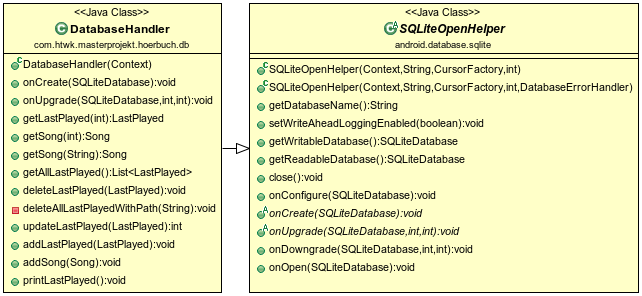
\includegraphics[scale=0.7]{images/database}
\caption{Klassen für die Implementierung der Datenbank}
\label{database}
\end{figure}
\end{center}

diese methode nennt sich \textit{onUpgrade} und wird bei eben erwhäter versionserhöhun automatisch ausgeführt. in dieser methode sollten eine datenmegrierung durchgeführt werden oder alle bestehenden daten gelöscht werden und neue tabellen angelegt werden.

durhc diesen meschanismuss ist eine aktuallität des datenbanklayouts immer gegeben. in der abblindung \ref{database} sind die kalssen ersichtlich die es ermöglichen mit der datenbank zu komunizieren. für die verwendung der daten ist es ratsam objekte zu verwenden um abgefragte datensatze weiterzuverwenden oder datensätze zu gewinnen. ein solches objekt wird in abbildung \ref{dbmodel} dargestellt.

\begin{center}
\begin{figure}
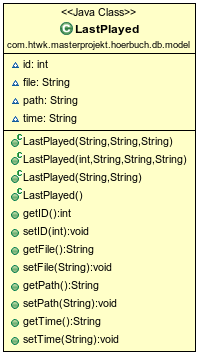
\includegraphics[scale=0.7]{images/dbmodel}
\caption{Obejkt zum transport der datensätze}
\label{dbmodel}
\end{figure}
\end{center}

\subsubsection{Abfragen}
Eine datenbankabfrage wird über einen sql befehl an die datenbank gestellt. Mit dem befehl \textit{SELECT} und der angabe der tabelle können daten aus der datenbank abgefragt werden. die abfrage wird dafür in ien Cursor Objekt geladen und der cursor anschließden zur ausführung an die datenbank gesendet.

das curser objekt enthällt anshcließend alle abgefragten daten welche die datenbank zum übergeben sql behel gefunden wurde. eine direkte abfrage ist nicht möglich.

es muss immer eine Curserobjekt verwendet werden. möchte man nur bestimtme datenban oder zielgerichtet daten aus der datenbank laden wird dme curser eine filterung mitgeteilt welche von der datenbank bei der abfrage der daten berücksichtigt wird.

das curserobjekt enthält eine lsite von allen dateneinträgen die geufnden wurde sind mehre datensätze gefunden wurden können diese durchlaufen werden und jeder datensatz einzeil betrachtet undverarbeitet werden.

bei der abfrage der einzelnen felder des datensatzes ist es nötig den datentyp der einzelnen daten zu kennen. das curserobjekt hat verschiedene mehtoden um untershciedliche datentypen aus den flender zu lesenen. diese typen können wie schon erwähnt nciht typsicher abgefragt werden. so sit es möglich ein datenfeld des types Integer in eine variable des Typen String zu laden.

der zugriff der datnebank kann über eine schreib oder lesbare datenbank gewährt werden. eine kombination sit nicht möglich. ein zugang zur datenbank kann entwerden nur shcrieben doer nur lesend sein.

möchte man schrieben und lesen wird die durch einen schreibenden zugriff und anschließen über einen lesenden zugriff realisiert. diese beiden vorgänge müssen sepratal initiiert wernden.

\subsubsection{Löschen}
das löschen von daten erfolgt ebenso wie das selektieren nach durch sql befehle anders wie bei dem slektieren existiert hierführ kein curser. es wird jedidlich mitgeteilt welcher datensatz in welcher tabelle gelöscht werden soll.

\subsubsection{Ändern}
ähnlich verhölt es sihc mit den ändern von datensätzen. hierführ wird der datenbank mitgeteilt welcher datensatz geändert werden soll und welche datenfelder mit welchem wert gesetzt werden soll.

die referenzierung einzelner datensätze erfolgt über primärschlüssel oder andere datenfelder, welche im sql behel angegebenw erden muss.

\subsubsection{Einfügen}
das anlegen neure datensätze verläuft durch die methode \textit{insert} diese methode verlangt ein lsite von schlüssel-wert-parren um eien datensatz anlegen zu können.

die lsite von paaren repräsentiert den eigentlichen datensetz. in ihr wirden alle datenfelder und die dazugehörigen werte abgelegt. ausgeschlossen ist der primärschlüssel dieser wird durhc einen trigger ind er datenbank automatishc erzeugt und beim einfügen in die datenbank automatisch im datensatz gespeichert.

der emtho wird nun die lsite mit den daten übergeben un die tabelle genannt , in der die daten abgeleggt werden soll.
